\section{The first algorithm: random walk}

A random walk on $G$ is a Markov chain over all vertices with the transition matrix:
\begin{equation*}
    P(w|v) = \begin{cases} 
      \frac{1}{r_v} & \text{if } $(v, w)$ \text{ is an edge.} \\
      0 & \text{o.w.}
   \end{cases}
\end{equation*}

where $r_v$ is the degree of the node $v$.

\begin{algorithm}
\caption*{$\textsc{Algorithm I \cite{aldous1990random} \cite{broder1989generating}}$}
\begin{algorithmic}
%\State Construct a probabililty distribution $\{p_e\}_{e\in E_G}$
%\INDENT
    \State  Simulate a simple random walk on the graph G starting at an arbitrary vertex $s$ until every vertex is visited. For each vertex $i \in V - s$ collect the edge $\{j, i\}$ that corresponds to the first entrance to vertex $i$. Let $T$ be this collection of edges. Output $T$.
%\ENDINDENT
\end{algorithmic}
\end{algorithm}
Our first algorithm is that a random walk can simulate a uniform spanning tree by selecting the first edge that enters the node. The pseudocode is shown above. The running time of Algorithm I is $O(mn)$. It's clear that $T$ is a spanning tree because it contains $|V|-1$ edges and no loops. We shall prove that it is indeed uniformly distributed. 

Before discussing the algorithm, it will be useful to introduce \emph{arborescences} defined as below:
\begin{definition}{(Arborescence)}    
    For a given $s \in G$, an arborescence $T$ \emph{rooted at $s$} is a directed spanning tree of $G$ where all vertices in $G \setminus \set{s}$ have \emph{exactly one} incoming arc.
\end{definition}

It is easy to check that there is a one-to-one correspondence between spanning trees of $G$ and arborescences rooted at $s$: given any spanning tree, there is a unique way of directing its edges to make it an arborescence rooted at $s$; conversely, given any arborescence rooted at $s$, one can obtain a spanning tree by simply disregarding the direction of the edges.
Therefore, if we get a procedure that generates arborescences, it also gives a procedure that generates spanning trees. 

Indeed, random walk simulates a chain of arborescences along the way.

\begin{definition}{(Arborescence chain).}
Let $(X_j; -\infty < j < \infty)$ be the Markov chain of a random walk on $G$. We can define a Markov chain of arborescences $(S_j; -\infty < j < \infty)$. Considering $(X_j, X_{j+1}, \cdots)$, we choose $X_j$ to be the root of $S_j$ and select the first edge entering other vertices to be in the tree. In other words, the tree $S_j$ is rooted at $X_j$ with edges $(X_{T_v^j - 1}, X_{T_v^j}); v \neq X_j$, where $T_v^j = \min \{k \leq j; X_k = v\}$. An example is given in Figure \ref{fig:example-forward}.
\label{def:forward}
\end{definition}

%\textbf{Example.} 
\begin{table}[h]
\centering
\begin{tabular}{llllllll}
0 & 1 & 2 & 3 & 4 & 5 & 6 & 7 $\cdots$\\ \hline
1 & 2 & 1 & 3 & 4 & 1 & 3 & 2 $\cdots$ 
\end{tabular}
\end{table}

\begin{figure}[h]
    \centering
    \subfloat[\centering $G$]{{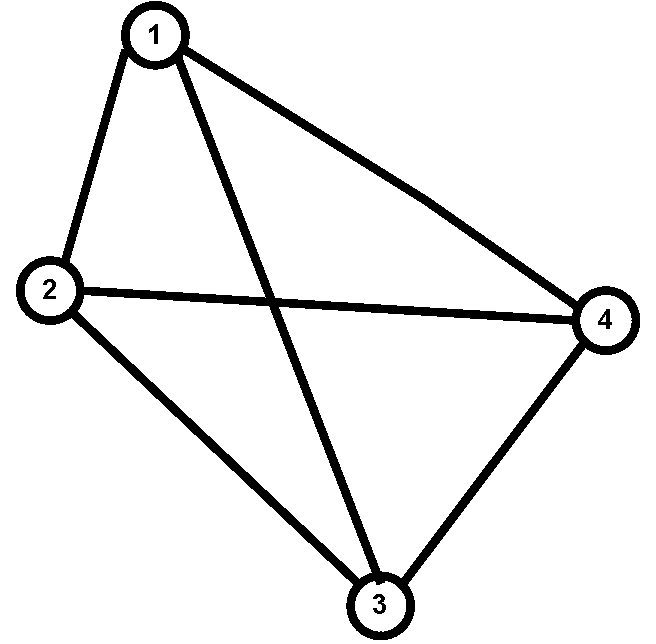
\includegraphics[width=.25\textwidth]{whole_graph.pdf} }}%
    \qquad
    \subfloat[\centering $S_0$]{{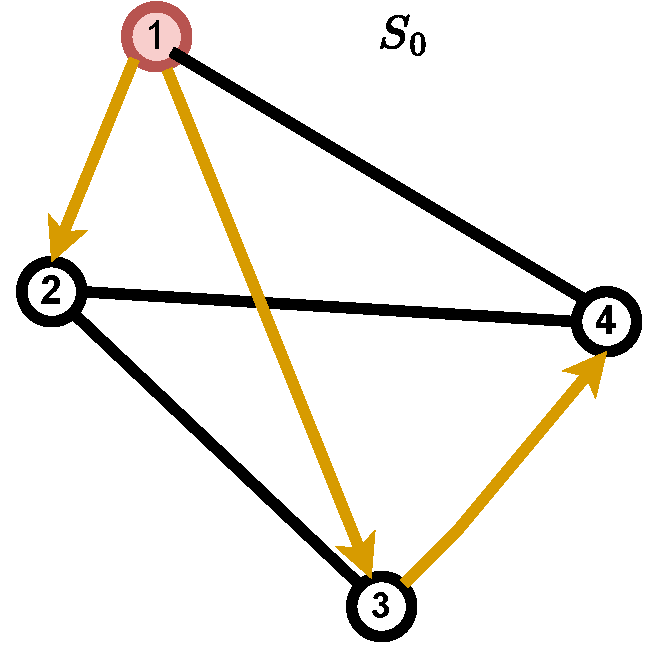
\includegraphics[width=.25\textwidth]{graph_0.pdf} }}%
    \qquad
    \subfloat[\centering $S_3$]{{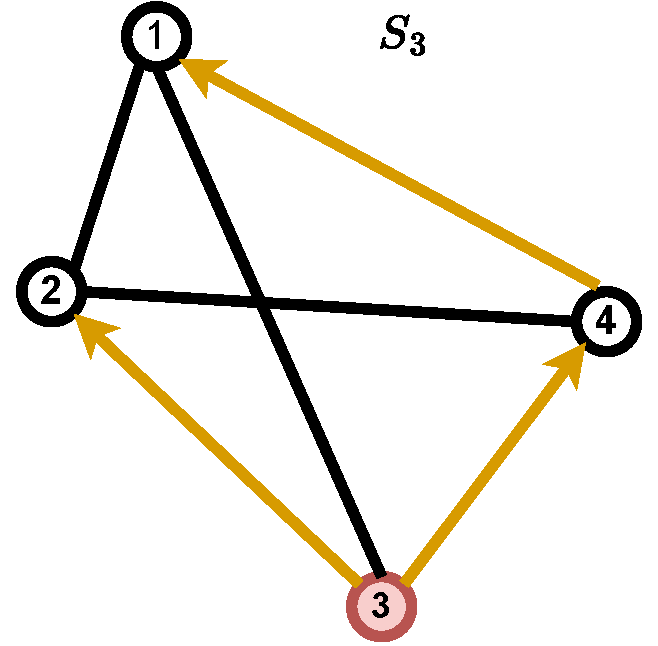
\includegraphics[width=.25\textwidth]{graph_3.pdf} }}%
    \caption{An example of an arborescene chain. The table above is a random walk over graph $G$. Then by Definition \ref{def:forward}, $S_0 = \{[1, 2], [1, 3], [3, 4]\}$ and $S_3 = \{[3, 4], [4,1], [3,2] \}$}%
    \label{fig:example-forward}%
\end{figure}


\begin{proposition}
   $(S_j; -\infty < j < \infty)$ is an irreducible and reversible Markov chain. 
\end{proposition}

\begin{proof}
Irreducibility and reversibility are directly from the assumption that $G$ is connected and unweighted. 
\end{proof}


\begin{theorem}
    Let $N(G)$ be the number of spanning trees $t$ of $G$. Then
$P(T = t) = 1/N(G)$ for each $t$ produced by Algorithm 1.
\end{theorem} 

We will first prove a simpler case when the graph is r-regular. 


\begin{proof}
    Let $G$ be an r-regular graph. Let $(X_j; -\infty < j < \infty)$ and $(S_j; -\infty < j < \infty)$ be the Markov chain of the nodes and arborescences introduced previously. 

Consider the transition matrix $Q$ for $S_j$ in reversed time:
$$Q(t, t') = P(S_{-1} = t' | S_0 = t)$$

Then
\begin{itemize}
    \item Given $t$, there are exactly $r$ trees $t'$ such that $Q(t, t') = \frac{1}{r}$ and $Q(t, t') = 0$ for other trees. 
    \item Given $t'$, there are exactly $r$ trees $t$ such that $Q(t, t') = \frac{1}{r}$ and $Q(t, t') = 0$ for other trees. 
\end{itemize}

This is because $X_{-1}$ has $\frac{1}{r}$ probability to be each of the $r$ neighbours of $v$. Each possibility leads to $S_{-1}$ being some tree $t'$, and these also are the only possibilities. A similar argument can be made going from $S_{-1}$ to $S_0$. Therefore, $Q$ is doubly-stochastic, which further implies that the stationary distribution of $S_j$ is uniform. 
\end{proof}

To extend the above proof to non-regular graphs, we first make the observation that each tree $t$ has $r(v)$ neighbours, where $v$ is the root of the tree. This implies that we can swap $r$ in the two bullet points above with the degree of the roots. It then follows that the stationary distribution of $t$ is proportional to the degree of its root. Thus, all directed spanning trees rooted at the same node are uniform. Since our trees are undirected and unrooted, all $T$ in Algorithm 1 are uniform. 